\chapter{Computational Methodology}
\label{ch:methods}
\section{Architecture and Training}
The flow network maps $(x,y,R_{\rm in},R_{\rm out},\Rey)$ to $(u,v,p)$
through five hidden layers of 70 tanh units. The force network maps the eight
inputs in \cref{eq:force-network} to two force components through five hidden
layers of 90 tanh units. Spatial coordinates are affinely normalized, and
the pressure output uses a scale $p_s=2L/h^2$.

\begin{figure}[p]\centering
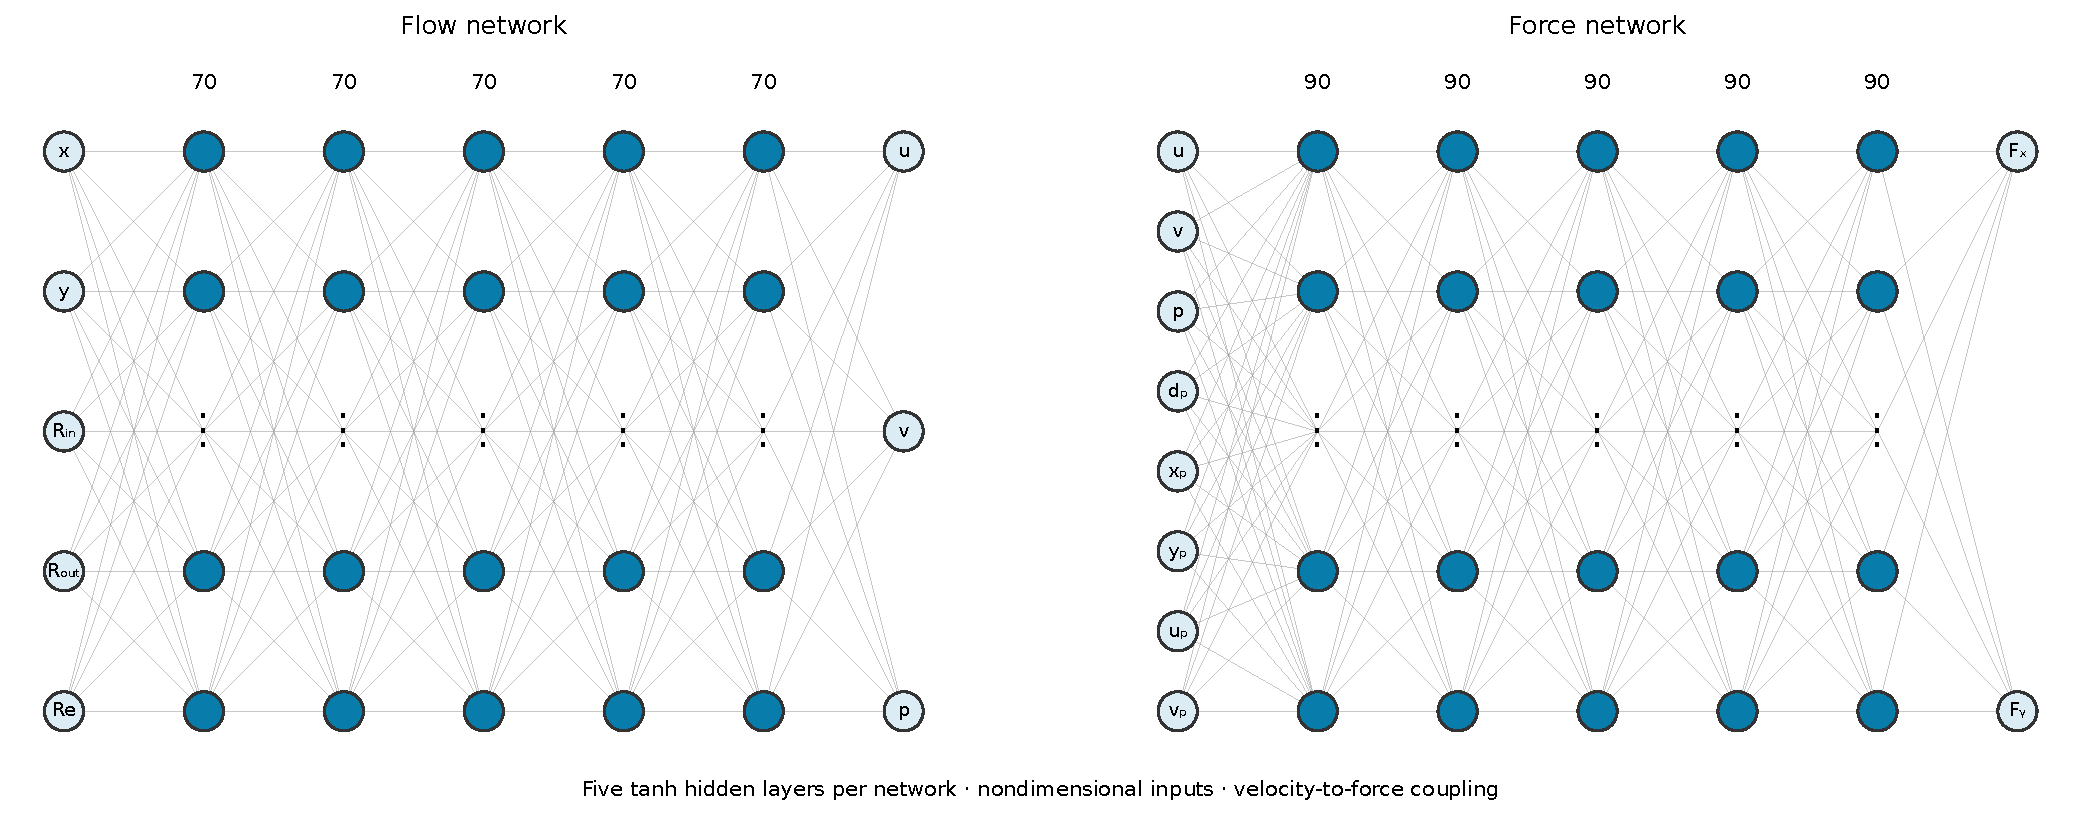
\includegraphics[width=.9\textwidth,trim=0 22 499.535 0,clip]{02_architecture.pdf}\par
\vspace{2mm}
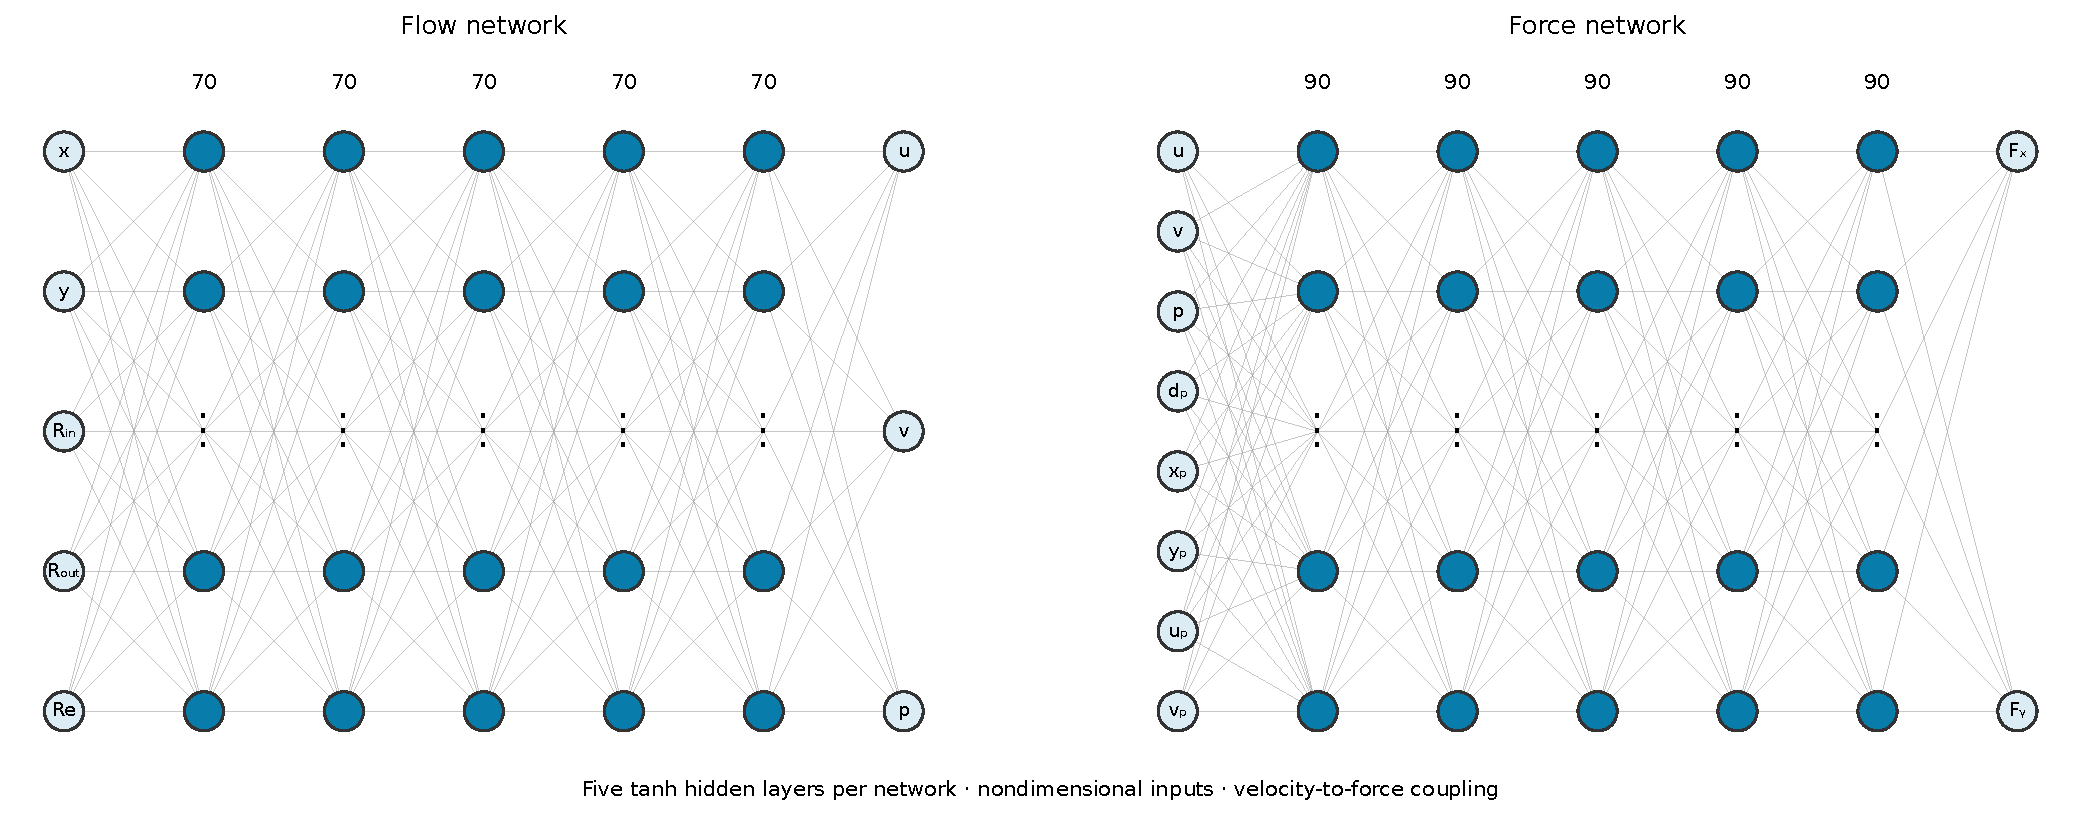
\includegraphics[width=.9\textwidth,trim=499.535 22 0 0,clip]{02_architecture.pdf}
\caption[Network architecture]{Flow network (top) and force network (bottom),
shown as enlarged crops of the existing architecture PDF. Five hidden
layers contain 70 and 90 units, respectively. Dots abbreviate neurons;
labels give actual layer widths.}\label{fig:architecture}
\end{figure}

For continuity residual $r_c$ and the two momentum residuals $\vect{r}_m$,
the implemented flow objective is
\begin{align}
 \mathcal L_{\rm flow}={}&\MSE(h r_c)+\MSE(h^2\vect{r}_m)
 +20\MSE(\widehat{\vect{u}}-\vect{u}_{\rm BC})\nonumber\\
 &+(\widehat p_g/p_s)^2
 +5\MSE(Q/Q_0-1).
 \label{eq:flow-loss}
\end{align}
Here the gauge pressure target is zero, and flux is sampled on seven sections
using 25 transverse points per section. This integral mass constraint helps
exclude a low-throughput interior field that would be inconsistent with
the prescribed inlet flux. The force loss is the mean-square residual
between normalized predicted drag and fluid--particle slip.

Interior samples are resampled during Adam training. Fixed PDE-monitor
samples support checkpoint selection, followed by L-BFGS refinement on
fixed collocation samples. Reference FEM interior labels do not enter the
flow-training objective. Each geometry/Reynolds-number case is trained
separately; fixed parameter input slots are not evidence of a parametric
solution across untrained geometries.

\begin{table}[!htbp]
\centering\small
\caption{Recorded settings of the preliminary training run.}
\label{tab:training}
\begin{tabularx}{\textwidth}{@{}lY@{}}
\toprule Item & Recorded setting\\\midrule
Principal flow seeds & 42 and 43; first seed used for the principal comparison\\
Initial flow phase & 1,000 Adam epochs, 512 interior samples per epoch, 250 L-BFGS iteration budget\\
Refinement phase & 1,800 Adam epochs, 1,024 samples per epoch, 700 L-BFGS iteration budget\\
Adam learning rate & $10^{-3}$ with cosine scheduling to $5\times10^{-5}$ per flow phase\\
Force training & 1,000 Adam epochs; batches of 512; learning rate $8\times10^{-4}$\\
Force selection and testing & 1,024 selection samples; separately sampled held-out tests\\
Flow evaluation & 1,600 fixed interior points for direct FEM comparison\\
3D manufactured benchmark & 800 Adam epochs and 400 L-BFGS iteration budget; a separate model\\
\bottomrule
\end{tabularx}
\end{table}
These settings describe the original training recorded in the checkpoint
metadata. The archived final study reloaded those weights to reproduce
evaluation and figures; its default command-line preset fields should not
be mistaken for a second training run.

\section{Independent FEM Reference}
The reference solves \cref{eq:continuity,eq:momentum} on a triangular mesh
constructed from the same centerline and width. Vector P2 velocity and P1
pressure spaces form the Taylor--Hood discretization
\cite{taylor1973,gustafsson2020}. Picard iteration treats the nonlinear
advection term, and each mixed linear system is solved with a sparse direct
solver. The finest recorded mesh has \FinestTriangles\ triangles. Identical
velocity conditions are imposed at the walls and both end sections; the
arbitrary pressure constant is fixed separately.

The curved wall is polygonal in the reference mesh, so mesh refinement
changes both discretization and geometric approximation. Three resolutions
are retained rather than treating a single successful solve as exact.
For repeated trajectory evaluations, a fast interpolator operates in the
channel's longitudinal/transverse coordinates. This prevents interpolation
across the hole inside a bend. Its error is measured against direct FEM
evaluation before trajectory comparisons are interpreted.

\section{Trajectory Integration and Cases}
ODE integration uses RK45 when the relaxation time is sufficiently long
relative to the geometric step limit, and Radau for shorter, stiffer
relaxation scales. The current tolerances are $2\times10^{-6}$ relative and
$2\times10^{-8}$ absolute. Event functions detect wall contact, outlet
crossing and inlet backflow; time and evaluation budgets keep each run
bounded. A failed path remains marked as failed. A finite output is never
silently replaced by the reference trajectory.

The principal particle has $d_p=\BaselineDiameter$ and
$\rho_r=\BaselineDensity$. Seven inlet positions span $\eta=-0.65$ to
$0.65$. Diameter cases use $d_p=0.0105,0.0255,0.045$, and density cases use
$\rho_r=200,1000,3000$. The baseline and the $\rho_r=1000$ control are
deliberately repeated in the output records and are not independent
physical replications.

Three comparisons isolate different error sources:
\begin{enumerate}
\item PINN flow with ForceNet versus FEM flow with exact Stokes drag measures
the complete surrogate transport discrepancy.
\item PINN flow with ForceNet versus the same PINN flow with exact Stokes
drag isolates the force-surrogate contribution.
\item Fluid markers in PINN and FEM fields examine flow-path differences
without particle inertia.
\end{enumerate}
The archive contains \TotalIntegrations\ integrations:
\ParticleIntegrations\ particle trajectories and \TracerIntegrations\
fluid-marker trajectories. They share models and inputs, and are not treated
as independent experimental observations.

\section{Data Provenance and Independence}
All current flow, force, and trajectory data are computational. The principal
evaluation seed is fixed rather than selected by the smallest FEM error.
The two-seed statistics describe observed training variability, with no claim
of a confidence interval or population-level inference. The current study
is developmental: seeing its failures informs the proposed research plan.
A new frozen evaluation set will therefore be used before making final
claims about improvements, as specified in \cref{ch:plan}.
